\chapter{Focus sur des sous parties du modèle}

\section{Structure des activités agropastorales}

Les participants ont fait le choix de distinguer les rôles de pasteur et d'agriculteur tout en soulignant qu'ils pouvaient tout à fait être endossés par la même personne. Nous y reviendrons plus loin, mais il est intéressant de constater qu'une grande part des conflits sont le fait des divergences d'intérêt de ces deux rôles. La superpositions des deux rôles en un même acteur (agro-pasteur) concourt à une plus grande stabilité du système et au partage d'une certaine empathie, les enjeux des deux rôles étant accessibles à la même personne.

Dans la figure \ref{fig:agripasteur} nous nous sommes intéressés aux réseaux égocentrés de l'agriculteur et de l'éleveur. Nous nous intéressons donc aux connexions directes que ces deux rôles entretiennent.

Les agriculteurs, comme les éleveurs, font partie des cuisines qui sont elles-mêmes sous l'autorité du chef de cuisine et du chef de concession. Ces deux rôles participent et contribuent à assurer la paix sociale.

Cette paix sociale en temps qu'élément liant du système est importante à caractériser, tant pour l'analyse du système que du point de vue des acteurs qui le constituent : les participants ont volontiers considéré la paix sociale comme un outil de production. Cette paix sociale est également territorialisée, et l'intensité des comportements qui s'y rapporte varie en conformité avec la première loi de la géographie de Tobler : “tout interagit avec tout, mais ce qui est proche interagit plus encore”, ce qui renforce l'interdépendance entre les acteurs/actants du réseau local de Diohine, ceux-ci vivant et travaillant dans la même zone géographique.

Lors d'évènements rituels annuels, les rôles d'éleveur et d'agriculteur sont en relation avec ceux des Saltigués et des Vieilles Mamans qui leur font des prédictions et mettent en œuvre des moyens de protection des personnes et des champs pour l'année à venir, lors de la grande chasse (c.f. section \ref{sec:premierchasse}).

\begin{figure}
  \begin{center}
    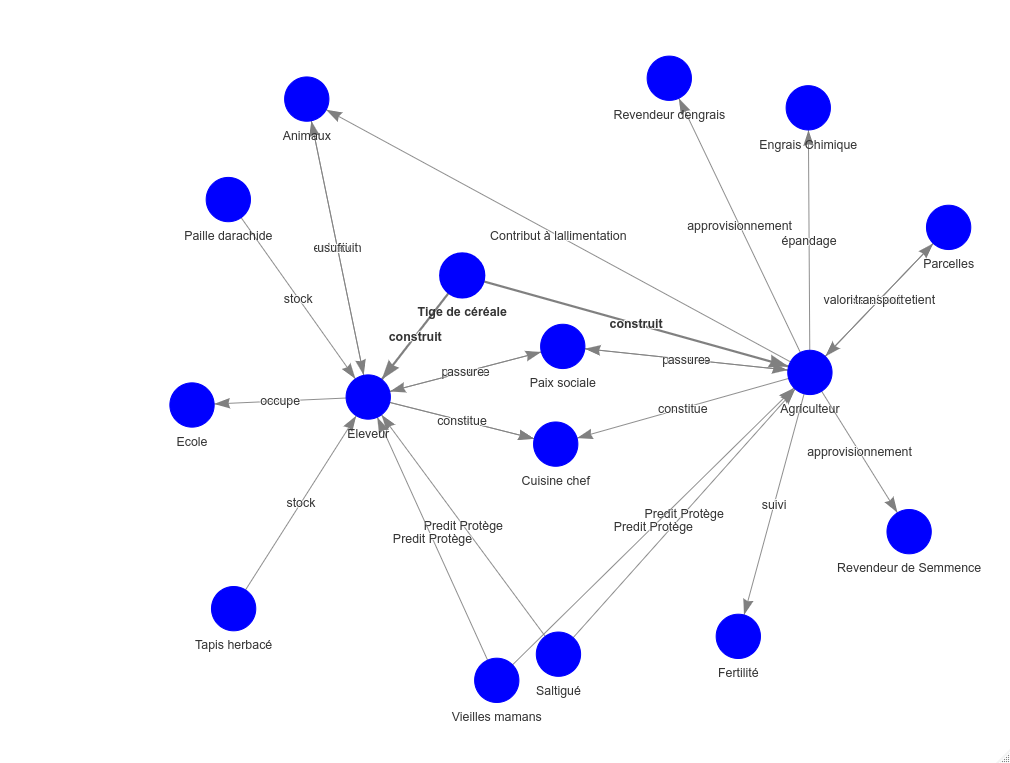
\includegraphics[width=0.9\textwidth]{img/agriculteur_eleveur.png}
  \end{center}
    %légende de l'image
  \caption{Sélections des relations entre agriculteur et éleveurs}
  \label{fig:agripasteur}
\end{figure}

\subsection{L'agriculteur}
C'est lui qui s'occupe, prend soin et valorise la terre. Il a des interactions avec les revendeurs de semences et d'engrais chimique, même si ces derniers ne sont pas assez disponibles.

La fertilité de la terre est un enjeu très important. Elle est suivie et perçue par les agriculteurs. L'exemple du quartier de Diohine qui s'est retiré temporairement de la jachère communautaire est éclairant à ce sujet :

Les habitants d'un quartier de Diohine voulaient pouvoir disposer de toutes leurs terres pour cultiver, y compris les parcelles en normalement jachère. Ils ont décidé de sortir de la jachère, ce qui peut s'expliquer par le fait car il n'y avait pas beaucoup d'éleveurs parmi eux, ils étaient donc moins sensibles aux enjeux de pâturage du bétail.

Au bout de trois ans, ils ont réintégré la jachère du quartier et les processus collectifs d'orientation des cultures qui l'accompagnent.
Les participants avancent deux types d'explication à ce revirement: d'une part la baisse des rendements constatés sur les parcelles sorties de la jachère, et d'autre part la XXXXX [TODO étienne remplir avec les raison d'Idrissa sur le statut social des ]


L'agriculteur contribue à l'alimentation des animaux de l'éleveur en mettant à disposition les résidus de culture, que ce soit directement sur la parcelle ou sous forme de bottes pailles de céréales récoltées.

\subsection{L'éleveur}
L'éleveur est défini par les fonctions qui le lie aux animaux. Il les entretient et bénéficie de l'usufruit de l'élevage. L'éleveur est également lié aux pailles de céréale et au tapis herbacé par la fonction de stockage qui servira plus tard à nourrir les animaux.

Par ailleurs un élément qui n'est pas visible sur le graphe est le lien qui existe entre le rôle d'agriculteur et celui d'éleveur. En effet dans la plupart des cas ces deux rôles sont occupés par la même personne. Mais quand l'agriculteur n'est pas éleveur, il confie des animaux à ce dernier qui a la charge de les entretenir et de les faire fructifier. L'éleveur est alors le banquier de l'agriculteur. On l'a abordé avec les questions des conflits; les agriculteurs gardent une part de responsabilité si leurs animaux font des dégâts sous le gardiennage de l'éleveur, ce qui accentue encore la relation de dépendance. Enfin on pourra souligner que tout le bétail d'un agriculteur n'est pas forcément confié au même éleveur. Ce qui permet d'accroître également les interdépendances.\\

Un élément particulièrement important constitue le lien entre les agriculteurs et les éleveurs : la paix sociale. C'est un concept auquel les acteurs se réfèrent souvent.

La paix sociale est un commun clef du système. Pour Aubert \textit{et al.} \cite{land_tenure_and_development_technical_committee_opportunities_2017}, un commun clé est "celui [ou ceux] susceptible d’avoir un effet d’entraînement important sur la résilience des autres communs qui lui sont liés". Ici, les éleveurs et les agriculteurs ont des intérêts qui peuvent diverger. Si un déséquilibre survient, la communauté fera le nécessaire pour restaurer la paix sociale et assurer sont maintient dans le temps.

Les participants considèrent la paix sociale comme un outil de production territorialisé. C'est un outil de production, car elle joue un rôle dans le bon fonctionnement de la communauté et permet le maintien dans le temps du système productif. Elle est territorialisée parce que la première loi de la géographie (voir plus haut) y joue à plein. Les liens qui unissent les acteurs sont très forts, et d'autant plus forts qu'ils sont entretenus dans le temps et dans l'espace.

\section{Structure de la résolution de conflit}

Nous avons voulu mettre un éclairage particulier sur la ou les structures de résolution de conflit. Ces conflits sont très majoritairement liés à la terre et aux fonctions et enjeux parfois contradictoires de l'élevage et de l'agriculture.

J.P. Jacob\cite{jacob_terres_2007}, considère que les droits fonciers en Afrique sont à considérer comme une manière de rattacher les humains et non humains à l'existence. Ces droits fonciers traditionnels lient moins les surfaces que le droit à l'existence des actants en mettant la priorité à l'inclusion plutôt qu'à l'exclusion. Considérer le droit foncier comme moyen d'existence fait le lien avec "la zone critique" que définit Latour\cite{latour_face_2015}. Cette dynamique contribue donc à repousser la vision individualiste de la modernité qui place l'autonomie au centre de tout. Or de manière curieuse, cette autonomie individuelle des modernes, ne tient pas du tout compte du réseau de solidarité entre humains et non humains qui la rend possible, et nie l'autonomie a laquelle une société peut prétendre collectivement.

Pourtant, et nous nous  attachons à le montrer dans la description des structures de résolution de conflit à Diohine, la prise en compte des réseaux de solidarité est omniprésente. Paul Séné nous dira même "ici nous dépendons tellement les uns des autres qu'on est bien moins libre que vous". Selon nous, la liberté dont parle Paul est en fait la recherche d'autonomie individuelle des modernes.


Nous avons extrait du diagramme général (fig. \ref{diagComplet}) la figure \ref{fig:conflict}

\begin{figure}
  \begin{center}
    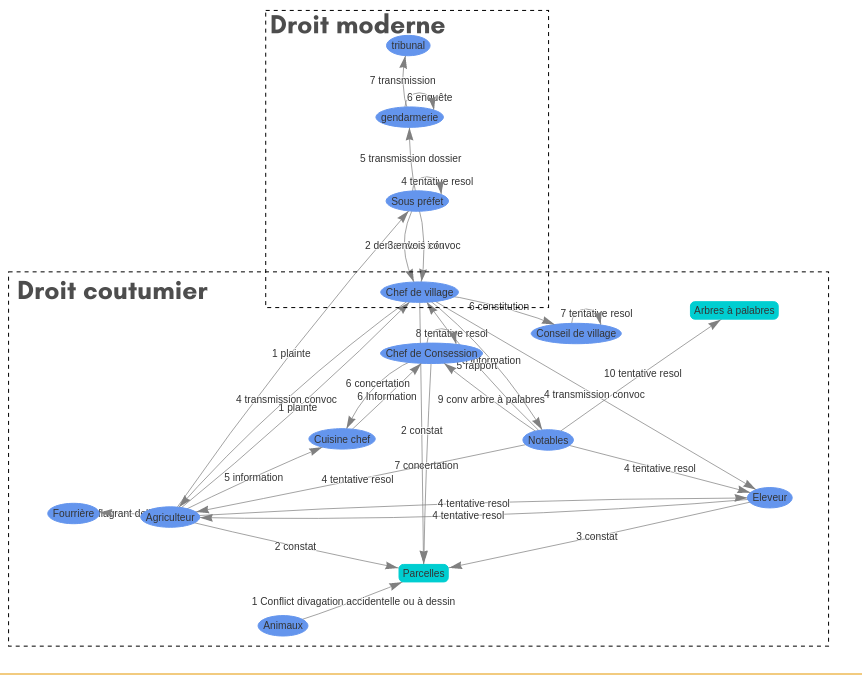
\includegraphics[width=0.9\textwidth]{img/zoneDroitConflits.png}
  \end{center}
  \caption{Selctions des relations liée au conflict. Extraction du sous-graphe des arcs étiquetés "dynamique conflit" du fichier}
  \label{fig:conflict}
\end{figure}

Deux ressources sont représentées sur ce sous-ensemble du modèle conceptuel : la parcelle, et l'arbre à palabre.

La parcelle est le support du droit à l'existence (J.P. Jacob). Le conflit va donc chercher à résoudre un dommage causé par A (ou via A': les objets de A) au droit d'existence de B. Toutes les tentatives de résolution du conflit (4 sur le schéma) impliquent des discussions et des concertations à chaque étage de la structure sociale.

Les animaux (A') de l'éleveur (A), ont causé des dommages sur la parcelle (B') de l'agriculteur B. L'agriculteur constate les dégâts, avec son chef de concession (au besoin). A et B vont tenter de résoudre le conflit sous l'autorité de leurs chefs de concession, si B refuse les compensations/amende honorables de A, le conflit est exposé au chef de village par l'intermédiaire du chef de concession. Le chef de village va pouvoir avoir recourt au Notable sous l'arbre a palabre de manière formelle ou informelle. À l'intégration de chaque nouvel acteur, B est sommé d'accepter la compensation de A pour rétablir la paix sociale. Si B se considère toujours lésé, il peut porter sa plainte auprès du sous-préfet. Celui-là peut demander l'avis rendu par le chef du village sur la base duquel il décide de transmettre le dossier à la gendarmerie qui établira une enquête avant de verser le dossier au tribunal.

Latour (La zone critque, 2021), rappelle la distinction entre  un \textit{monde où l'on vit} et un \textit{monde dont on vit}. Le monde où l'on vit  est l'endroit où l'on inscrit ses gestes du quotidien, alors que le monde dont on vit est  celui dont on dépend pour vivre, celui dont sont tirées les ressources et les objets qui supportent ces gestes quotidiens. [TODO etienne raccorder avec boite verte en dessous ]

Pour H. Arendt\cite{arendt_condition_2020} l'Homme est le plus souvant plongé dans le \textit{vita activa} (en oposition avec la \textit{vita contemplativa}). La \textit{vita activa} est elle même composé de trois éléments : le travail, l'\oe{}uvre et l'action. Le travail rassemble toutes les taches qui sont essentiel à la survie des individus; les choses qui leurs permettent de vivre et de perpétuer le cycle naturelle (manger, se déplacer, \textit{etc.}). L'\oe{}uvre est "l'activité qui correspond a la non naturalité de l'existance humaine[...]. L'\oe{}uvre fourni un monde artificiel, nettement différent du tout milieu naturel." (p. 58). Enfin l'action "correspond à la condition humaine de la pluralité, au fait [...] qu'ils [des hommes] vivent sur terre et habite le monde.[...] cette pluralité est spécifiquement \textit{la} condition [...] \textit{per quam} de toute vie politique."(p.60).

\todo{lien à faire avec vita activa (H.Arendt) Travail, oeuvre (tous les objets de l'environnement), action}

Cette distinction entre \textit{monde où l'on vit} et \textit{monde dont on vit} s'applique aux conflits de Diohine. Il y a deux échelles de résolution de conflit:  celle du monde où l'on vit qui s'étend jusqu'aux frontières du village et mobilise les acteurs locaux lors des tentatives de résolutions à l'amiable accompagnées par les notables et le chef de village selon les lois du droit coutumier,  et celle du monde dont on vit, qui s'étend au delà du village jusqu'aux instances d'autorité nationales et selon les lois du droit moderne positif.
Si on se place du point de vu du conflit, les acteurs locaux sont dans l'action au sens de H. Arendt, temps que le conflict est géré par la coutume. Quand il passe dans le droit conventionnel, le conflit se déplace dans la sphère du travail. Sa gestion est délégué en dehors du \textit{monde où l'on vit} 

Les acteurs organisés autour d’échelle de négociation locale et de l'arbre à palabre tentent par la concertation (\textit{Xartan} en Wolof) de résoudre le conflit. À chaque étape, `chef de concession`, `chef de village`, \textit{etc.} la victime est au centre de l'attention sociale. C'est à elle qu'il est demandé d'accepter l'amende honorable qui est faite par le contrevenant. Tant que ce n'est pas le cas, le contrevenant est exposé au niveau d'autorité supérieur.

\begin{quote}
    "Il est préférable de régler un problème assis plutôt que debout" (proverbe sérère). \textit{il vaut mieux que le problème se règle discrètement dans la cuisine plutôt que sous l'arbre a palabre}
\end{quote}


Quand le conflit dépasse le chef de village pour arriver au sous-préfet, le conflit sort du domaine du droit traditionnel pour entrer dans celui du droit positif. Et le droit Postif domine le droit traditionnel. On passe donc dans le domaine du monde dont on vit. Celui dont on dépend même à ses dépens.

Le fait que la très grande majorité des interactions se tienne  entre des  acteurs (seulement deux ressources sont identifiées), met en relief l'importance du "politique" et du langage au sens de H. Arendt\cite{arendt_condition_2020}. En effet, par le langage au sein des différentes instances de discussion/négociation des conflits, le résultat de l'action va évoluer de l'intention originale. "Cette contrainte exprime la dépendance de l'activité individuelle à l'égard du réseau de relation humaine" (p.43, Paul Ricoeur, in H. Arendt\cite{arendt_condition_2020}).

\section{Structure et mécanique de gestion collective de l'espace}

Le territoire de la commune de Diohine se distingue des communes voisines par la survivance d'une gestion collective de l'espace. Une partie des terres de la commune est chaque année mise en commun en temps que jachère collective. Cette jachère permet un repos de la terre, et laisse des espaces à la veine pâture.

\begin{figure}
  \begin{center}
    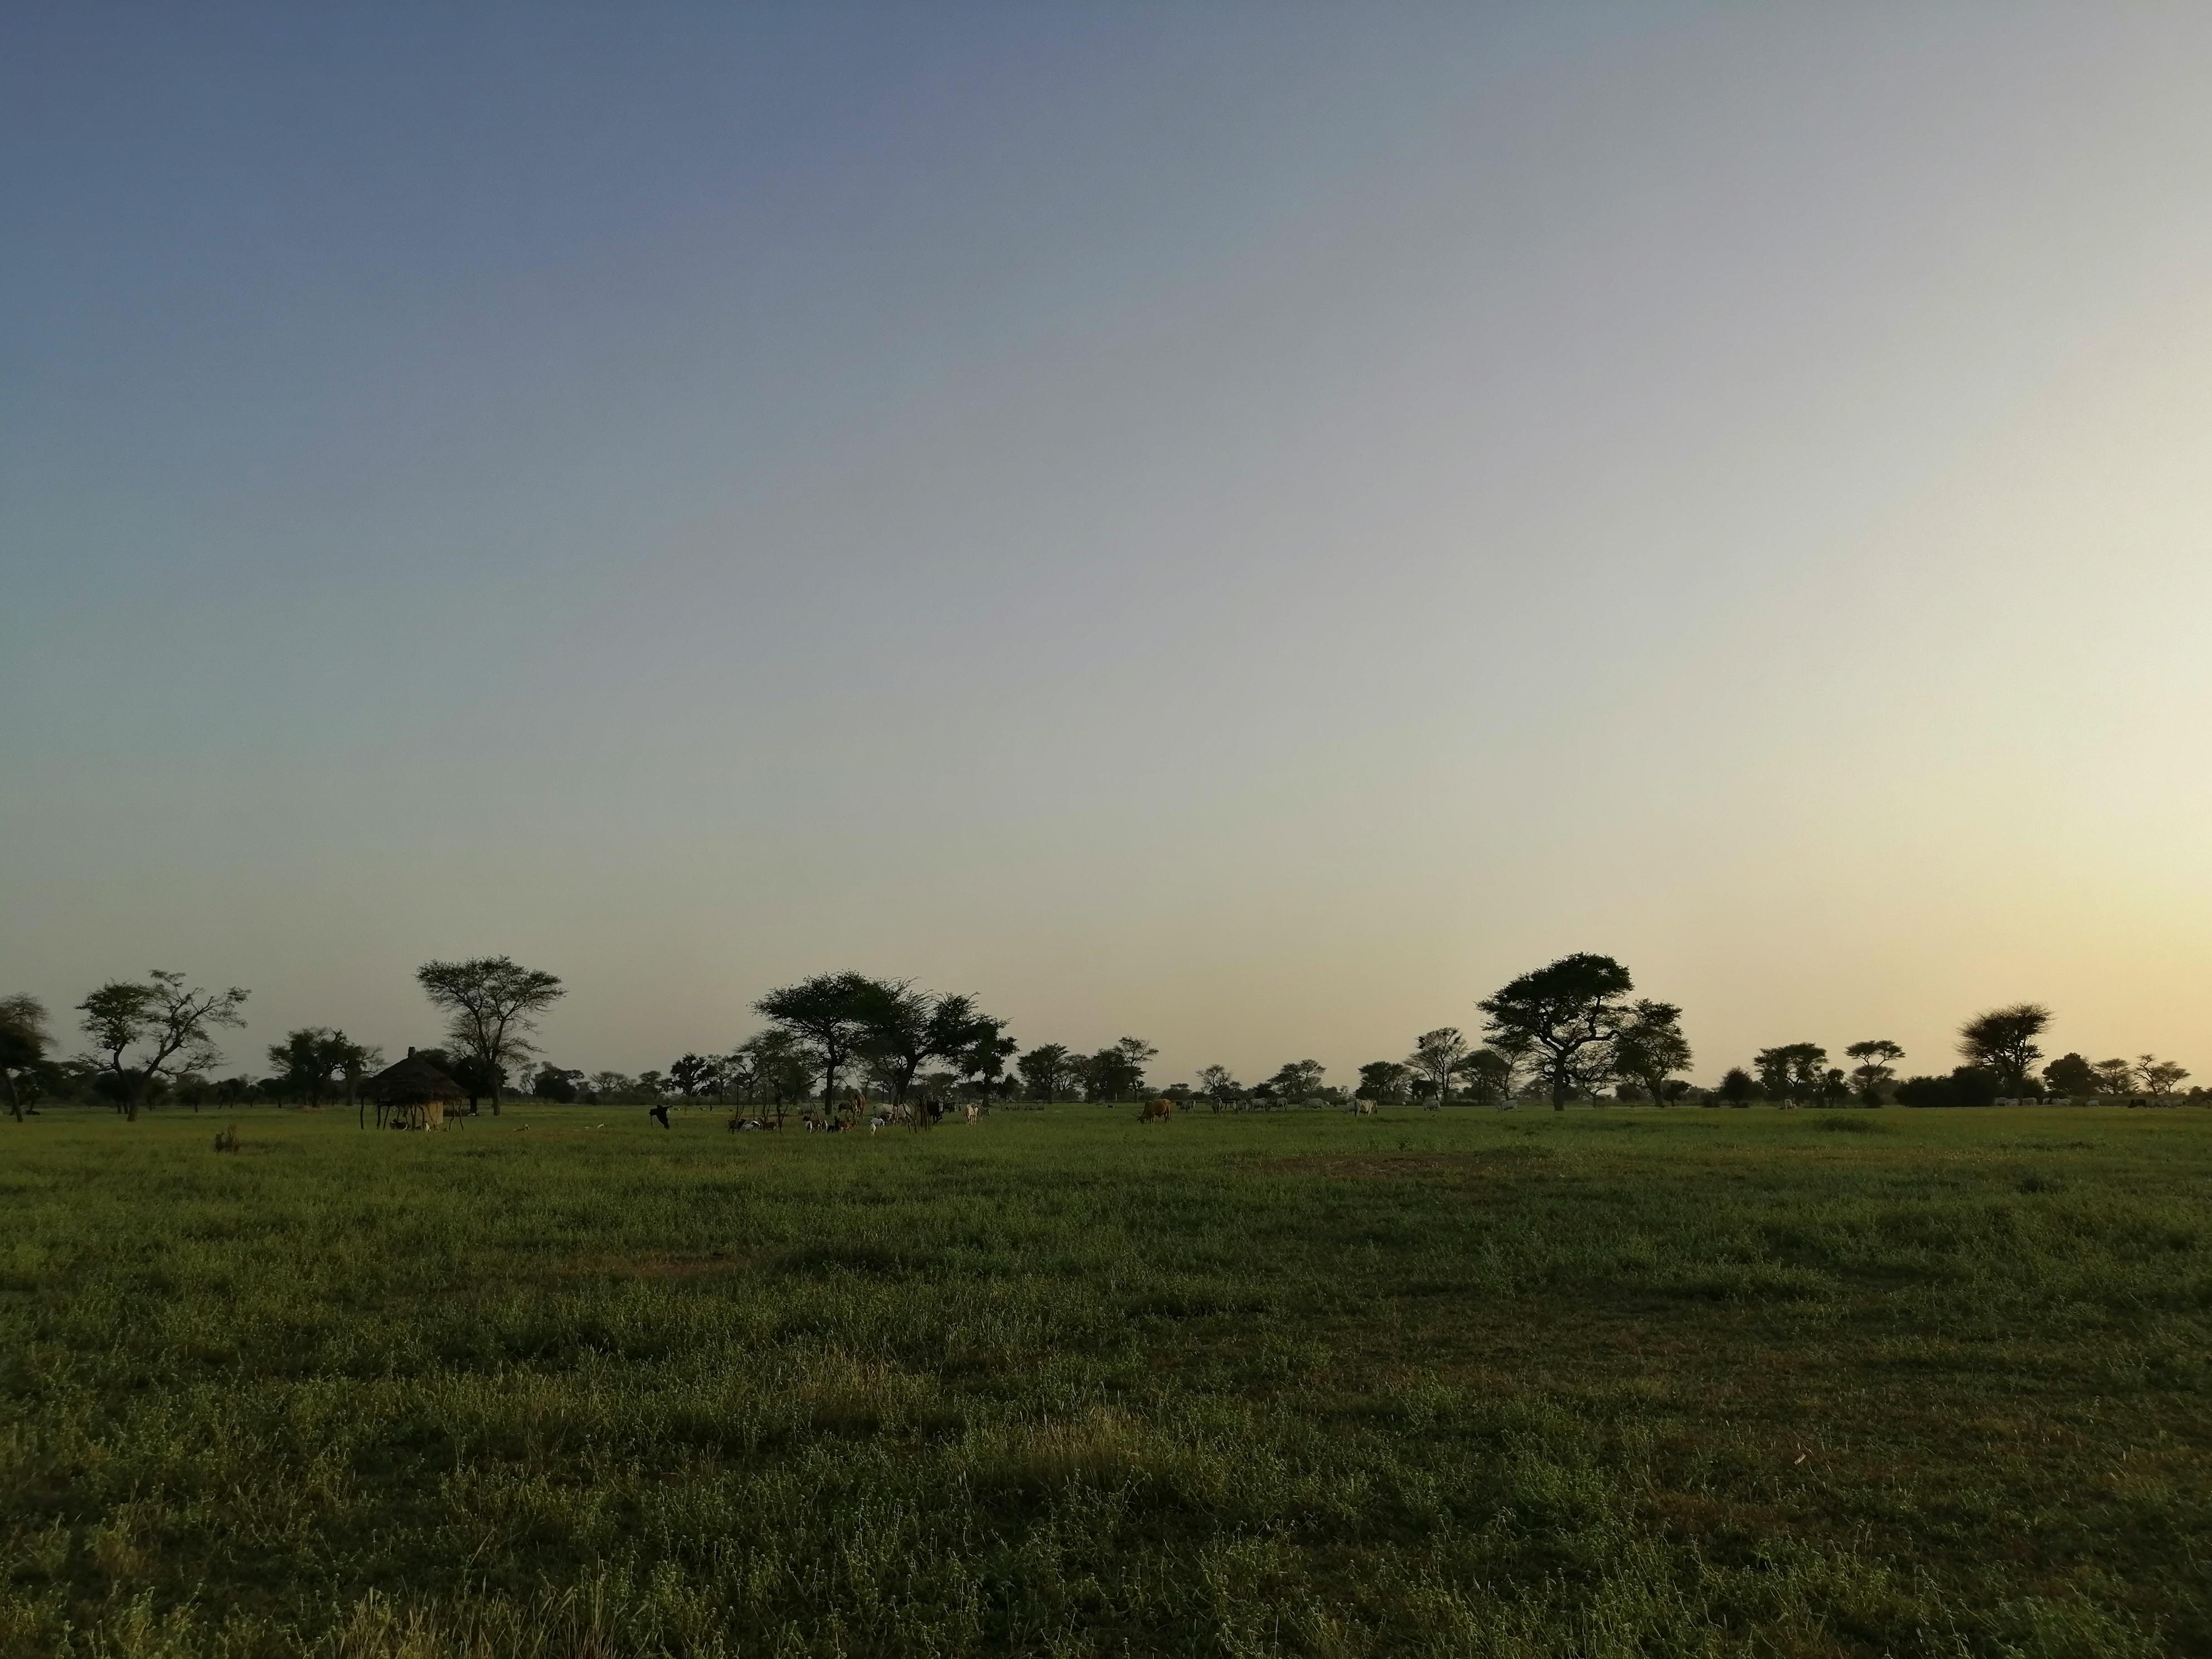
\includegraphics[width=0.9\textwidth]{img/jachere.jpg}
  \end{center}
    %légende de l'image
  \caption{Jachère au Nord de Diohine (photo prise en octorbe 2021)}
  \label{fig:photoJachere}
\end{figure}



Les animaux sont  sous la surveillance d'un berger la journée et sont attachés "au piquet" la nuit pour profiter des amendements liés à la fumure. Les animaux sont gardés la nuit, et le berger s'abrite dans une petite hutte (c.f. fig. \ref{fig:photoJachere})

Les espaces de jachère doivent être continus pour permettre aux animaux de se déplacer plus facilement et pour éviter les dégâts. Si une cuisine a un grand nombre de parcelles dans la jachère une année donnée, elle va se faire prêter ponctuellement des parcelles pour subvenir à ses besoins par les autres membres de la communauté.

La zone de jachère n'est pas une zone d'exclusion de la culture. On y inverse simplement la charge de la surveillance du bétail. Dans les zones cultivées, c'est au berger de faire attention à ce que le bétail ne rentre pas dans les parcelles. Si d'aventure une parcelle était mise en culture dans la jachère communautaire, la charge de la surveillance serait au cultivateur.

L'évolution de la démographie et des pratiques culturelles et culturales fait qu'aujourd'hui la jachère est régulièrement "rognée". Cette diminution des surfaces se fait par les bords qui sont moins exposés qu'une parcelle cultivée seule et entourée de jachère.

Pour les acteurs, la survivance de la jachère est en partie liée à l'histoire du peuplement de Diohine. Initialement constituer de peu de famille, les arrangements sont plus facile. Ces familles étaient assez homogènes en termes de pratique : tous agro-pasteurs. Il y a donc une conscience forte de l'importance du bétail pour restituer la fertilité aux champs.

La saison des cultures, et l'organisation du territoire qui en découle est lancé au moment de la première chasse. Seront définis à ce moment-là les espaces de culture, et c'est à partir de ce moment là que les prêts de parcelles pourront avoir lieu.

Extraction du sous graphe des arcs étiquetés  "interaction" du fichier DOT \url{https://github.com/ElCep/DSCATT/blob/master/PARDi/diagram_pardi_simple_edges.dot}

 \subsection{Mise en commun : la première chasse}\label{sec:premierchasse}



 \titlebox{\textit{Les saltigués}}{
   La cérémonie divinatoire du xooy est organisée à l’approche de la saison des pluies sur la place des villages par la communauté des Serer du centre-ouest du Sénégal. Durant cette longue veillée nocturne, les maîtres voyants, connus sous le nom de saltigués, se succèdent dans le cercle qui leur est réservé pour délivrer, au rythme des tamtams, leurs prédictions à une assistance en délire. La cérémonie du xooy apporte des réponses aux questions clés pour la communauté que sont, entre autres, la pluie, les fléaux ou les maladies et les remèdes.\footnote{Source : \href{https://ich.unesco.org/fr/RL/le-xooy-une-crmonie-divinatoire-chez-les-serer-du-sngal-00878}{site de l'unesco}.}
 }

Cet événement annuel est constitué de trois temps forts :
\begin{enumerate}
  \item La réunion nocturne, qui regroupe les hommes. Les voyants, "\textit{saltigués}", et ce «qui ont des dons », partagent leur prédiction, et leur connaissance sur l'année à venir, les grandes tendances, si des calamités sont à prévoir on identifie les solutions et les libations à faire. Ce sont ces infos qui seront centralisées par le grand saltigué.
  \item Première chasse. Elle concerne plusieurs villages.  Le grand \textit{saltigué} centralise les informations, des autres \textit{saltigués}et fait un message à tout le monde , avec des recommandations. Les hommes partent à la chasse dans la brousse, les anciens restent à discuter sous l'arbre à palabre. C'est un moment important de la transmission de connaissance, chaque quartier a un délégué qui rapporte au saltigué les informations sur sa zone, son quartier.
  \item La réunion diurne le même jour que la chasse a pour objet de définir les orientations des cultures et négociations d'accès à la terre. Il y a une réunion par quartier de Diohone et les informations sont ensuite centralisées. Et les zones de jachère, d'arachides et de mil sont définies.
\end{enumerate}

Il y a un enjeu fort à participer à la première chasse pour chaque cuisine, car le gibier sacré de l'année (e.g. un lièvre) sera partagé entre le/les premiers chasseurs. Le morceau de l'animal ramené dans la concession permettra de bénir les semences et d'assurer une bonne récolte.

Apris la chasse vient le défrichage  et  le jour des étrennes, on prépare une bière de mil et on se souhaite bonne fête.


\subsection{Interaction dyadiques : le prêt de terre}

Une fois que le zonage est effectué lors de la réunion diurne, les tractations pour obtenir des parcelles  peuvent commencer. Ce sont des négociations qui se font dans la discrétion des cuisines et sont très largement tributaires du réseau de solidarité que les uns et les autres sont capables de mobiliser (c.f. infra).

Les parcelles sont prêtées par le chef de cuisine, pour une durée d'un an. Les prêts étaient traditionnellement accompagnés d'offrande/cadeau en nature. Mais de plus en plus ces pratiques se métamorphosent en location (prêt contre de l'argent).

\section{Les réseaux de solidarité}

\titlebox{\textit{warning}}{
  Est-ce que la solidarité ici est proche/assimilable à la notion de proximité de l'école des proximités (Tores, Grossetti, Bouba-olga)

  [paul]Pour Grosseti que je situe vaguement, je pense qu'on peut parler d'encastrement, je ne connais pas l'école des proximités.

  [paul] Les interactions listées précédemment s'inscrivent dans différents réseaux de solidarité, solidarité étant ici entendue au sens de la relation qui peut exister entre des acteurs partageant le même contexte d'action collective, et reconnaissant l'obligation d'assistance qui lie les membres du groupe auquel ils appartiennent.

}



Différents réseaux de solidarité existent de manière imbriquée et enchâssée les uns dans les autres. Nous proposons de distinguer trois types de solidarités selon la nature des ressources qui fondent les interactions et leur portée.

On pourra d'abord distinguer des solidarités spatiales, de courte portée,  mobilisées lors des négociations et des discussions annuelles récurrentes ( prêt de terres en cas d'insuffisance, orientation des cultures, aménagement des couloirs pour le passage du bétail) ou ponctuelles ( garde de troupeau, prêt d'animal de trait, d'outil).
Ce réseau est un réseau qu'on pourrait qualifier de réseau de  voisinage, puisqu'il comprend les cuisines d'un même groupement de quartiers.

Le second réseau , qui se sur-impose au réseau de voisinage,  mobilise des acteurs plus éloignés : des  membres des cuisines d'autres groupements de quartiers.
Les interactions sont plus ponctuelles : conseils sur l'achat ou la vente de bétail, prêts d'argent, soin au bétail, renouvellement d'outils. Exemple : mobilisation générale du village pour cultiver et récolter en cas de maladie d'un paysan
Enfin un troisième réseau de solidarité , plus étendu, est celui qui lie les cuisines à leur famille lointaine, installée dans les villes  de taille plus importante , voire d'autres pays (diaspora).
Ce réseau est le support d'interactions  moins fréquentes , et il semblerait qu'il soit mobilisé principalement pour contribuer financièrement à la sécurité alimentaire des familles du village, ou à statuer sur des évènements politiques majeurs. (La diaspora mondiale peut même être convoquée pour certains évènements majeurs de la vie du village)
